\section{Introduction}

\frame{
   \frametitle{The lifetime frontier at the LHC}
   \begin{columns}
   	\column{0.6\textwidth}
   \begin{itemize}
   	\item Weakly coupled \textcolor{red}{long lived particles} (LLP) encompass all three other frontiers
   	 \vspace{0.4cm} 
   	 \item The SM already has templates for such particles ($\nu$, $K_L^0$, ...) 
   \end{itemize}
   \column{0.4\textwidth}
   	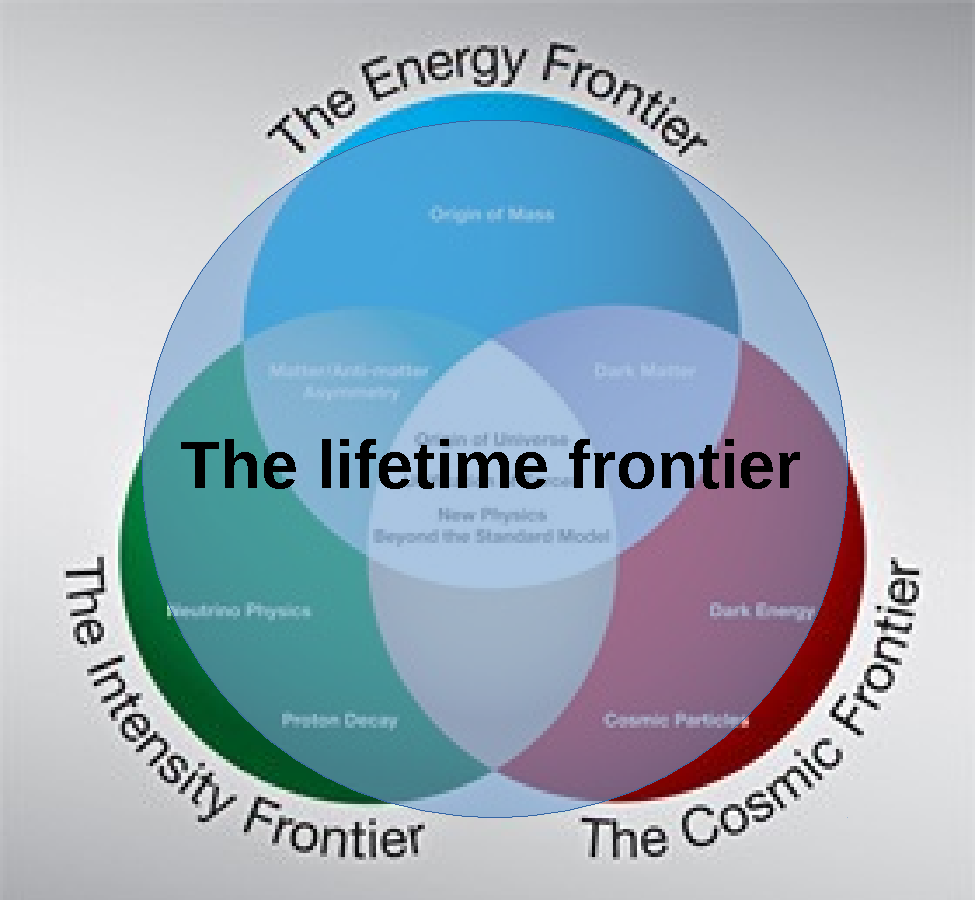
\includegraphics[width=1.3in]{figs/intro/lifetime_frontier}   	
   \end{columns}
\vspace{0.3cm}
   \begin{columns}
   		\column{0.45\textwidth}
   		\centering
   	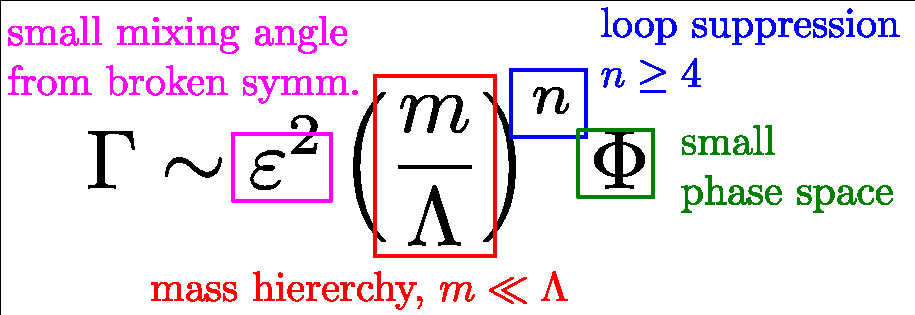
\includegraphics[width=2.1in]{figs/intro/lifetime_suppression} 
	\column{0.55\textwidth}
	\begin{itemize}
		\item Large lifetimes are driven by several factors
	\end{itemize}	
    \end{columns}
\vspace{0.3cm}

    \begin{itemize}
    	\item $pp$ collisions at LHC are excellent source of LLP's. But high $p_T$ (ATLAS/CMS) or restricted $c\tau$ (LHCb) searches can miss these.

    \end{itemize}
}

\frame{
	\frametitle{Cast a wide net}
	   \begin{columns}[T]
		\column{0.33\textwidth}
		\centering
		\includegraphics[width=1.6in]{figs/intro/Susy-particles}
		\column{0.33\textwidth}
		\centering
	    \includegraphics[width=0.7in]{figs/intro/dm}
		\column{0.33\textwidth}
		\centering
	    \includegraphics[width=1.5in]{figs/intro/other_llp}
	   \end{columns}	
   \scriptsize	
	   \begin{columns}[T]
	\column{0.33\textwidth}
\begin{itemize}
	\item[] R-parity violation
	\item[] Gauge mediated SUSY
	\item[] (mini-)split SUSY
	\item[] stealth SUSY
\end{itemize}
	\column{0.33\textwidth}
\begin{itemize}
	\item[] Asym. DM
	\item[] Freeze-in
	\item[] Composite DM
	\item[] Coannihilating DM
\end{itemize}
	\column{0.33\textwidth}
    \begin{itemize}
    	\item[] Baryogenesis
    	\item[] Neutrino masses
    	\item[] Neutral naturalness
    	\item[] Hidden Valleys
    \end{itemize}
\end{columns}
\vspace{0.5cm}
\normalsize
\begin{itemize}
	\item Lifetimes as long as sub-second-ish (BBN limit) possible
	\item Masses can range from sub-MeV to 100~GeV
\end{itemize}
}

\frame{
   \frametitle{LHCb perspective {\small [see also \href{https://indico.cern.ch/event/714087/timetable/\#5-lhcb-snapshot}{\textcolor{blue}{\tt Elena's}} talk]}}
  \begin{itemize}
  	\item Complementarity between ATLAS/CMS and LHCb: luminosity, acceptance, triggers, lifetime reach. 
  \end{itemize}
  \begin{center}
	    \includegraphics[width=2.5in]{figs/intro/lhcb_reach}
   \end{center}
   \vspace{-0.6cm}
   \begin{itemize}
   	\item Our best tracks originate inside the VeLo ($L\sim20$cm). Longer lifetimes are challenging.
   \end{itemize}
}

\frame{
	\frametitle{Other LLP detector proposals at the LHC}
   \begin{columns}
	\column{0.5\textwidth}
	\centering
    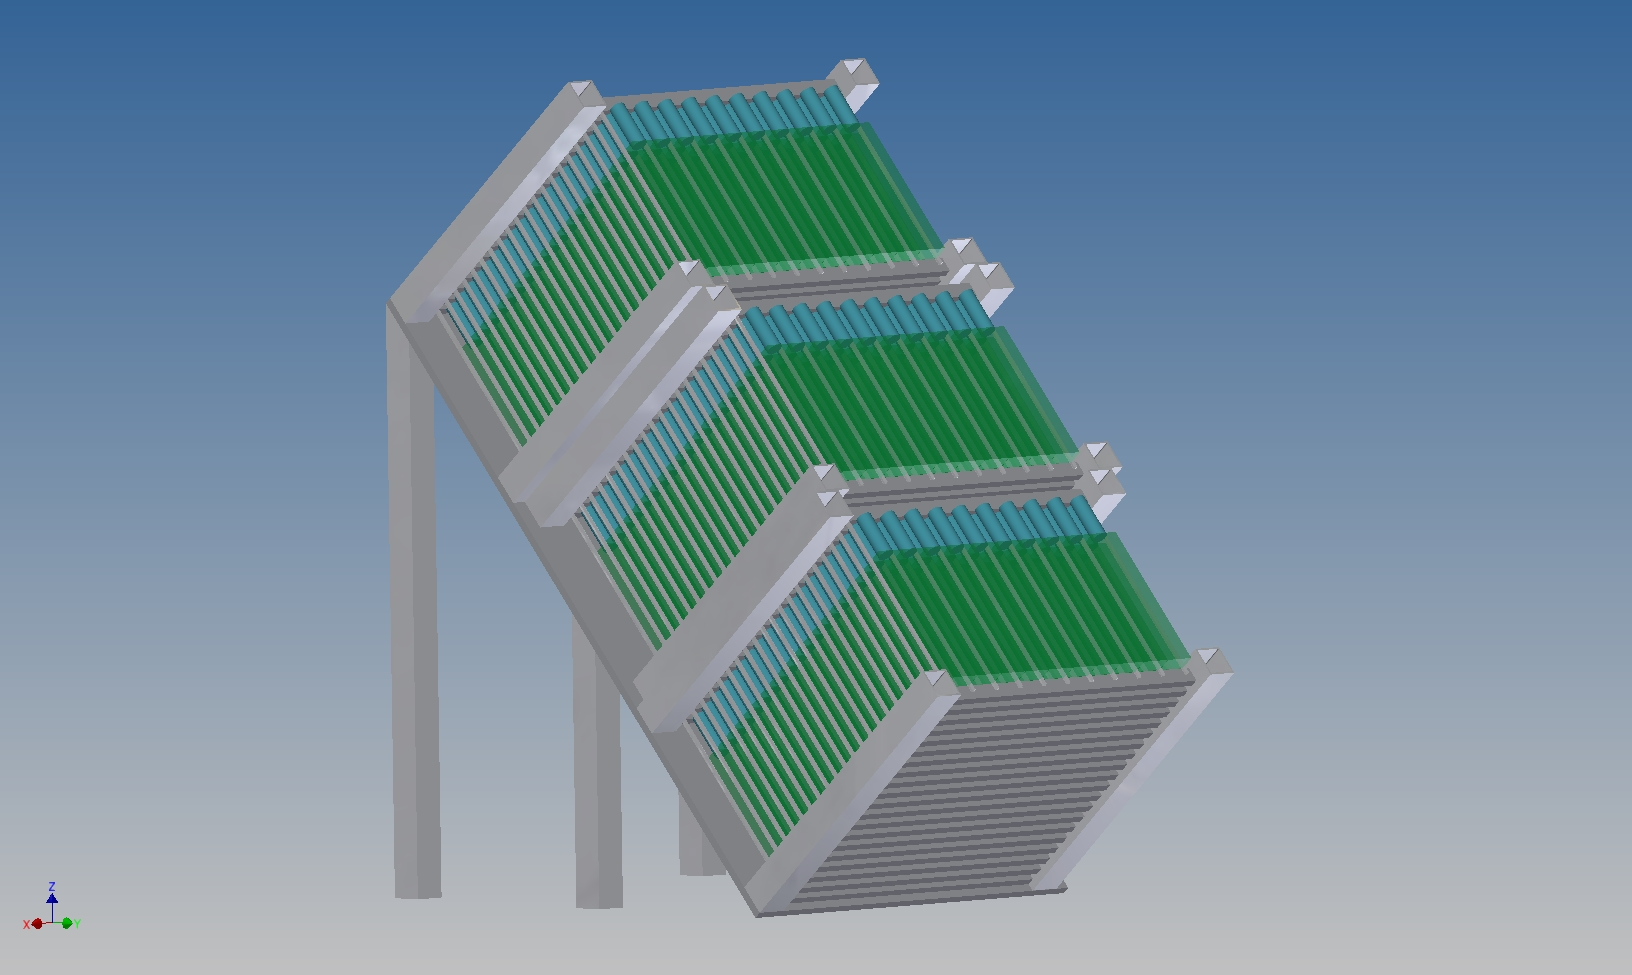
\includegraphics[width=1.9in]{figs/intro/milliqan}\\ {\tt MilliQan: \href{https://arxiv.org/abs/1607.04669}{\textcolor{blue}{1607.04669}}}
	\column{0.5\textwidth}
	\centering
	\vspace{-0.6cm}
	    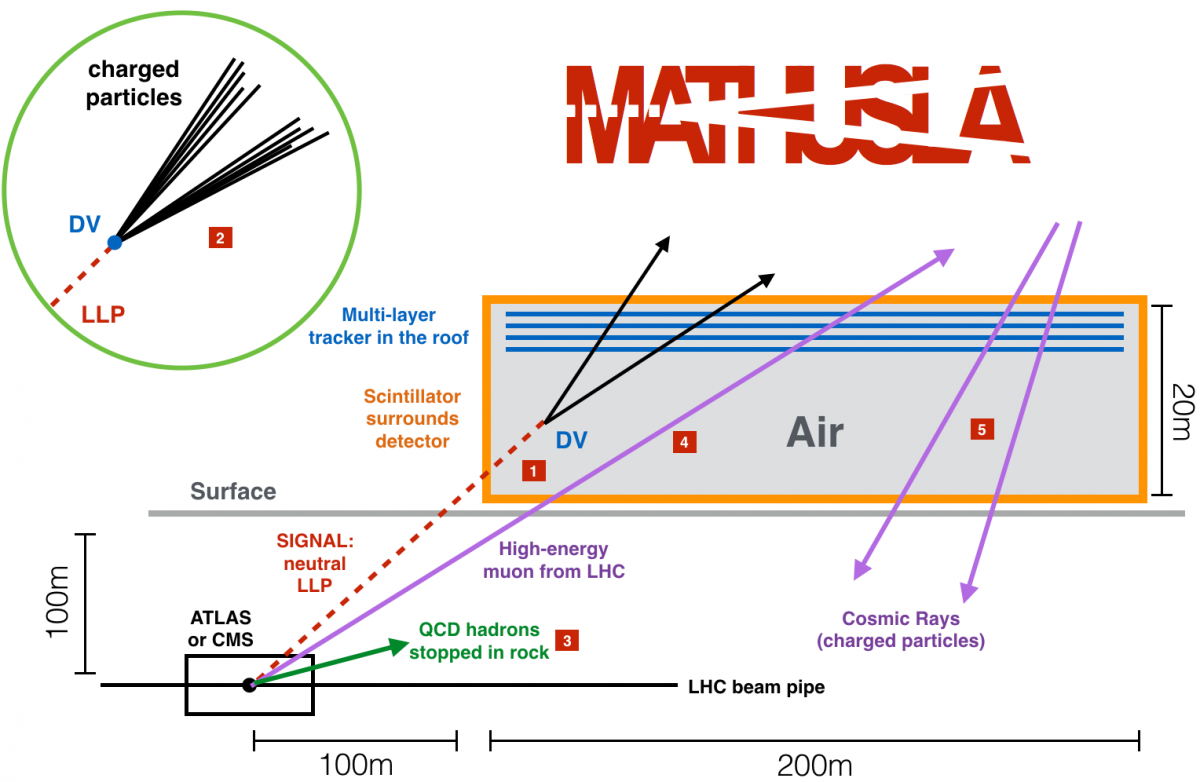
\includegraphics[width=1.9in]{figs/intro/mathusla}\\\vspace{0.4cm} {\tt MATHUSLA: \href{https://arxiv.org/abs/1606.06298}{\textcolor{blue}{1606.06298}}}
	\end{columns}
\vspace{0.5cm}
   \begin{columns}[T]
	\column{0.5\textwidth}
	\centering
	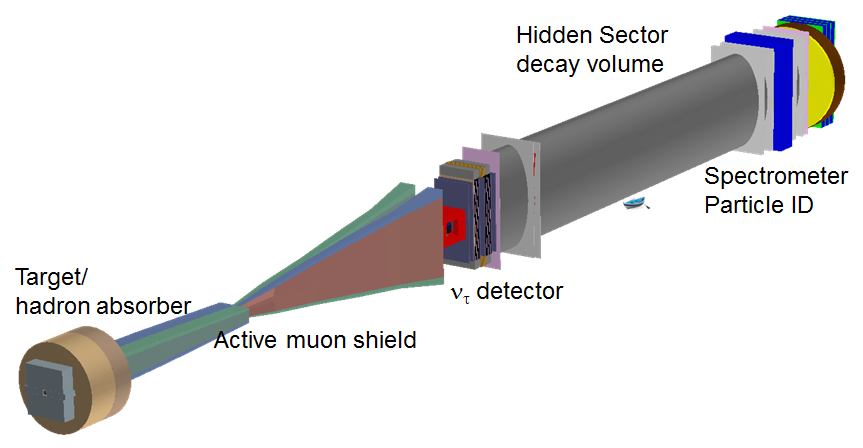
\includegraphics[width=1.78in]{figs/intro/ship}\\ {\tt SHiP: \href{https://arxiv.org/abs/1504.04855}{\textcolor{blue}{1504.04855}}}
	\column{0.5\textwidth}
	\centering
	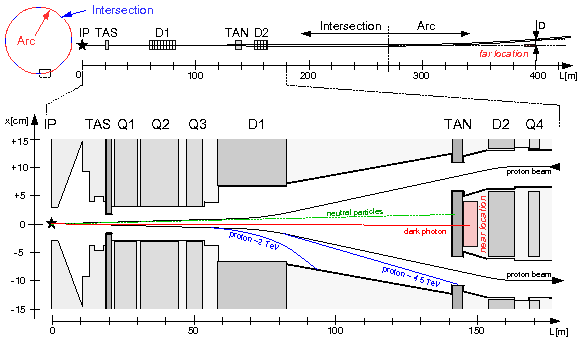
\includegraphics[width=1.6in]{figs/intro/faser}\\ {\tt FASER: \href{https://arxiv.org/abs/1708.09389}{\textcolor{blue}{1708.09389}}}
\end{columns}

}

\section{CODEX-b proposal}

\frame{
   \frametitle{CODEX-b: proposal at Point~8}
   \vspace{-0.3cm}
    \begin{center}
	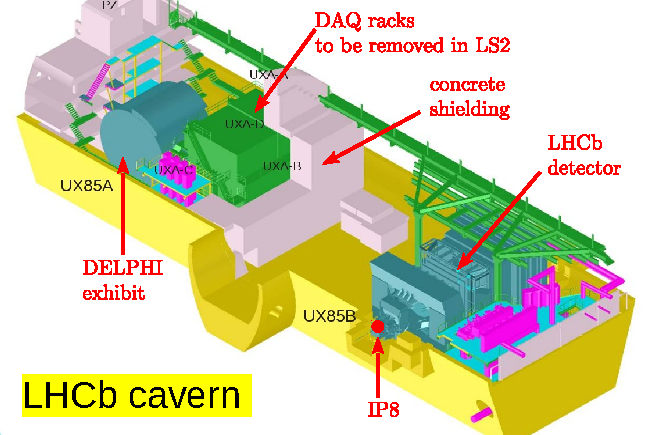
\includegraphics[width=3.5in]{figs/intro/lhcb_cavern}
	\end{center}
\vspace{-0.3cm}
    \begin{itemize}
    	\item DAQ racks in UXA-D move to surface for Run~3. Space available.
    	\item Shielded, underground, \textcolor{red}{$10\times10\times10$~m} box, around \textcolor{red}{$25$~m from IP}.
    	\item Instrument with tracking layers $\Rightarrow$ \textcolor{red}{CODEX-b}
    \end{itemize}
}


\frame{
	\frametitle{CODEX-b: another view}
    \begin{center}
	\includegraphics[width=3.9in]{figs/intro/codexb_box}
\end{center}   
\vspace{-0.5cm} 
    \begin{itemize}
	\item If DELPHI is removed, access to even $\textcolor{red}{20}\times10\times10$~m box.
	\item Angular acceptance $\sim 1\%$.
\end{itemize}
}

\frame{
	\frametitle{Minimal geometry for tracking}
	\vspace{-0.3cm}
   \begin{columns}[T]
	\column{0.5\textwidth}
	\centering
	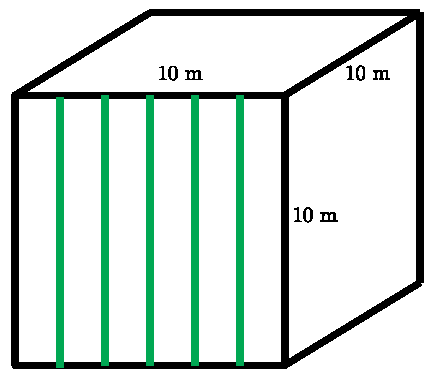
\includegraphics[width=2.3in]{figs/intro/codexb_box_poc}
	\column{0.5\textwidth}
	\centering
	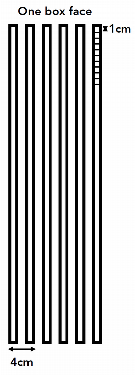
\includegraphics[width=0.8in]{figs/intro/codexb_box_poc_1}
    \end{columns}
\vspace{-0.2cm}
\small
    \begin{itemize}
    	\item \textcolor{red}{6 RPC layers} at 4~cm intervals on each box \textcolor{red}{face} with 1~cm granularity
    	\item \textcolor{DarkGreen}{5} equally spaced \textcolor{DarkGreen}{triplets} along the depth to minimize distance between reconstructed vertex and 1st measurement. $\epsilon_{\rm {\small tracking}}\sim \mathcal{O}(1)$.
    	\item \textcolor{blue}{50-100~ps} timing from RPC's foreseen for \textcolor{blue}{mass} reconstruction
    \end{itemize}
}

\frame{
   \frametitle{Why is CODEX-b attractive}
   \normalsize
   \begin{itemize}
   	\item Small volume to instrument. \textcolor{red}{Cheaper} and more leverage to try out additional calorimetry, 4d-tracking detectors
   	\vspace{0.4cm}
   	\item \textcolor{red}{Backgrounds} are controllable. Underground and existing shields. Space for additional shields
   	\vspace{0.4cm}
   	\item Only $\sim 4$ bunch-crossing away from IP8. With good timing (sub-$100$~ps), can \textcolor{red}{couple} with LHCb. Eg. tag a $B\to K^\ast \varphi$ between the two detectors.
   	\vspace{0.4cm}
   	\item \textcolor{red}{Complementarity} and competitive NP reach wrt other searches.
   \end{itemize}
}


\section{Backgrounds and shielding}

\frame{
   \frametitle{Minimal shield design}
   \begin{itemize}
   	\item CODEX-b sits behind the UXA (concrete) shield. From RP group, charged fluxes nominally quite low (access area!).
   \end{itemize}
   \begin{center}
   	\includegraphics[width=3.1in]{figs/intro/minimal_shields}
   \end{center}
   \begin{itemize}
   	\item Add passive \textcolor{red}{Pb shield} to attenuate muon and neutral hadrons. Thin \textcolor{red}{active veto} for secondaries inside the shield.
   \end{itemize}
}

\frame{
   \frametitle{Background studies: simulation}
    \begin{itemize}
	   \item Min. bias w/ {\tt Pythia8}. HL-LHC projections: 300/fb @ 14~TeV. 
	   \item Propagation thru' Pb, air and concrete in Geant4. 
    \end{itemize}
	   \begin{columns}[T]
	   		\column{0.52\textwidth}
	\centering
	\includegraphics[width=2.5in]{figs/intro/shield_veto_eff}
	\column{0.5\textwidth}
	\begin{itemize}
		\item Main remnant background is $n$.
		\vspace{0.15cm}
		\item Air-$\mu$ interactions vetoable by front detector face RPC's
		\vspace{0.15cm}
		\item Very little neutrino bkgd.
	\end{itemize}
    \end{columns}
    \vspace{0.35cm}
    \begin{itemize}
    	\item Track topology and timing will also help vetoing in the future.
    	\vspace{0.1cm}
        \item Study shows active veto suggests $\epsilon_{\rm veto} \sim 10^{-5}$ needed and doable.
    \end{itemize}
}


\frame{
   \frametitle{Background studies: simulation (cntd.)}
   	\begin{columns}
   	\column{0.4\textwidth}
   	\centering
   	\includegraphics[width=2in]{figs/intro/veto_energy_spectrum}
   	\column{0.6\textwidth}
   	    \begin{itemize}
   		\item Spectrum after veto is also soft. Expected multiple scattering is reduced.
   		\vspace{0.4cm}
   		\item Geant4 study broadly consistent with simplified propagation models with inputs from available data (PDG etc.).
   	\end{itemize}
   	\end{columns}
}

\frame{
	\frametitle{Background studies: validation measurements}
	\begin{columns}
   	\column{0.4\textwidth}
    \centering
    \includegraphics[width=2in]{figs/intro/muons_bkgd_noshield}
    \column{0.6\textwidth}
    \begin{itemize}
    	\item Neutrals are hard, but charged flux in the simulation can be \textcolor{red}{validated}.
    	\vspace{0.4cm}
    	\item Use to \textcolor{red}{calibrate} the simulation as well
    	\vspace{0.1cm}
    \end{itemize}
    \end{columns}
   \vspace{0.4cm}
    \begin{itemize}
    	\item Measure \textcolor{red}{charged flux} during current Run~2 \textcolor{red}{behind UXA} wall.
    	\vspace{0.3cm}
    	\item Later, more extensive measurements with different shield thickness, orientations, etc.
    \end{itemize}
}

\frame{
    \frametitle{Background studies: measurements (cntd.)}
	\begin{columns}
	\column{0.7\textwidth}
	  \begin{itemize}
	  	\item Two $30\times30\times2$~cm wrapped plastic scintillators + PMT + mechanical stand.
	  \end{itemize}
      \vspace{0.5cm}
      \centering
      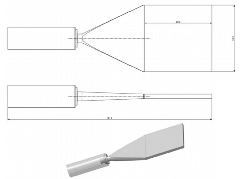
\includegraphics[width=2.3in]{figs/intro/scintillators}
	\column{0.3\textwidth}
	    \centering
	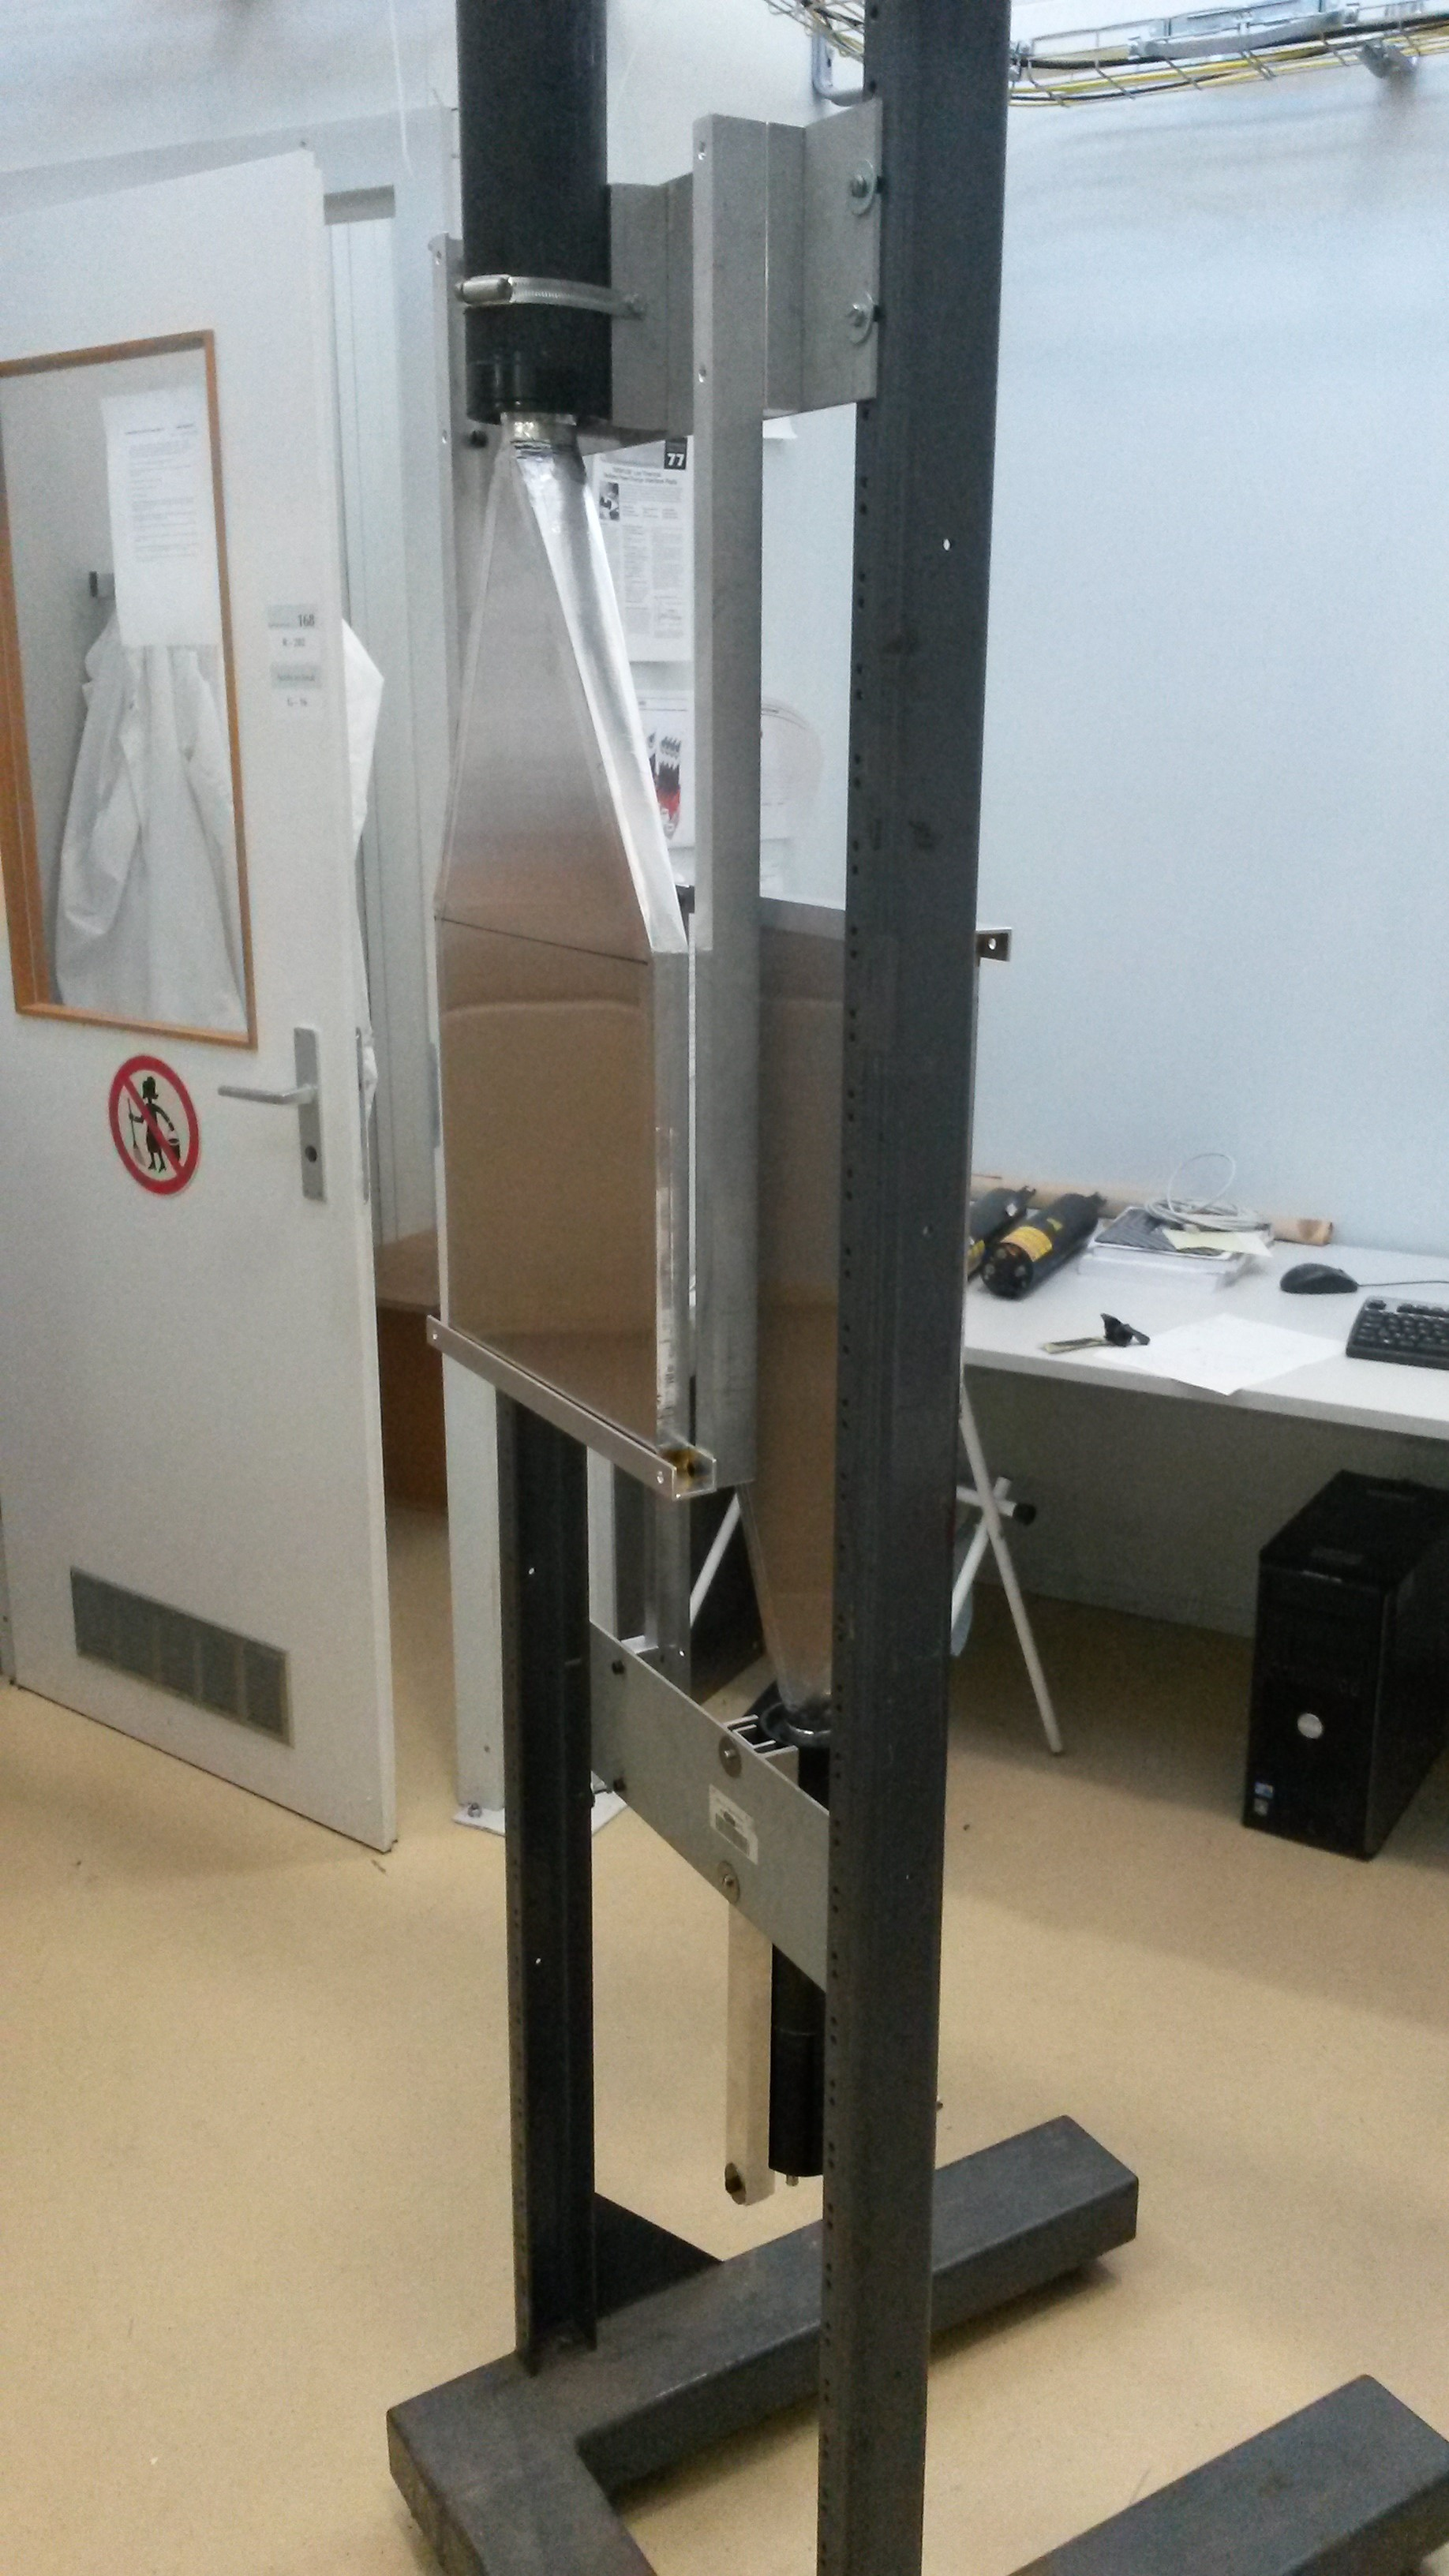
\includegraphics[width=0.8in]{figs/intro/mechanical_stand}\\
	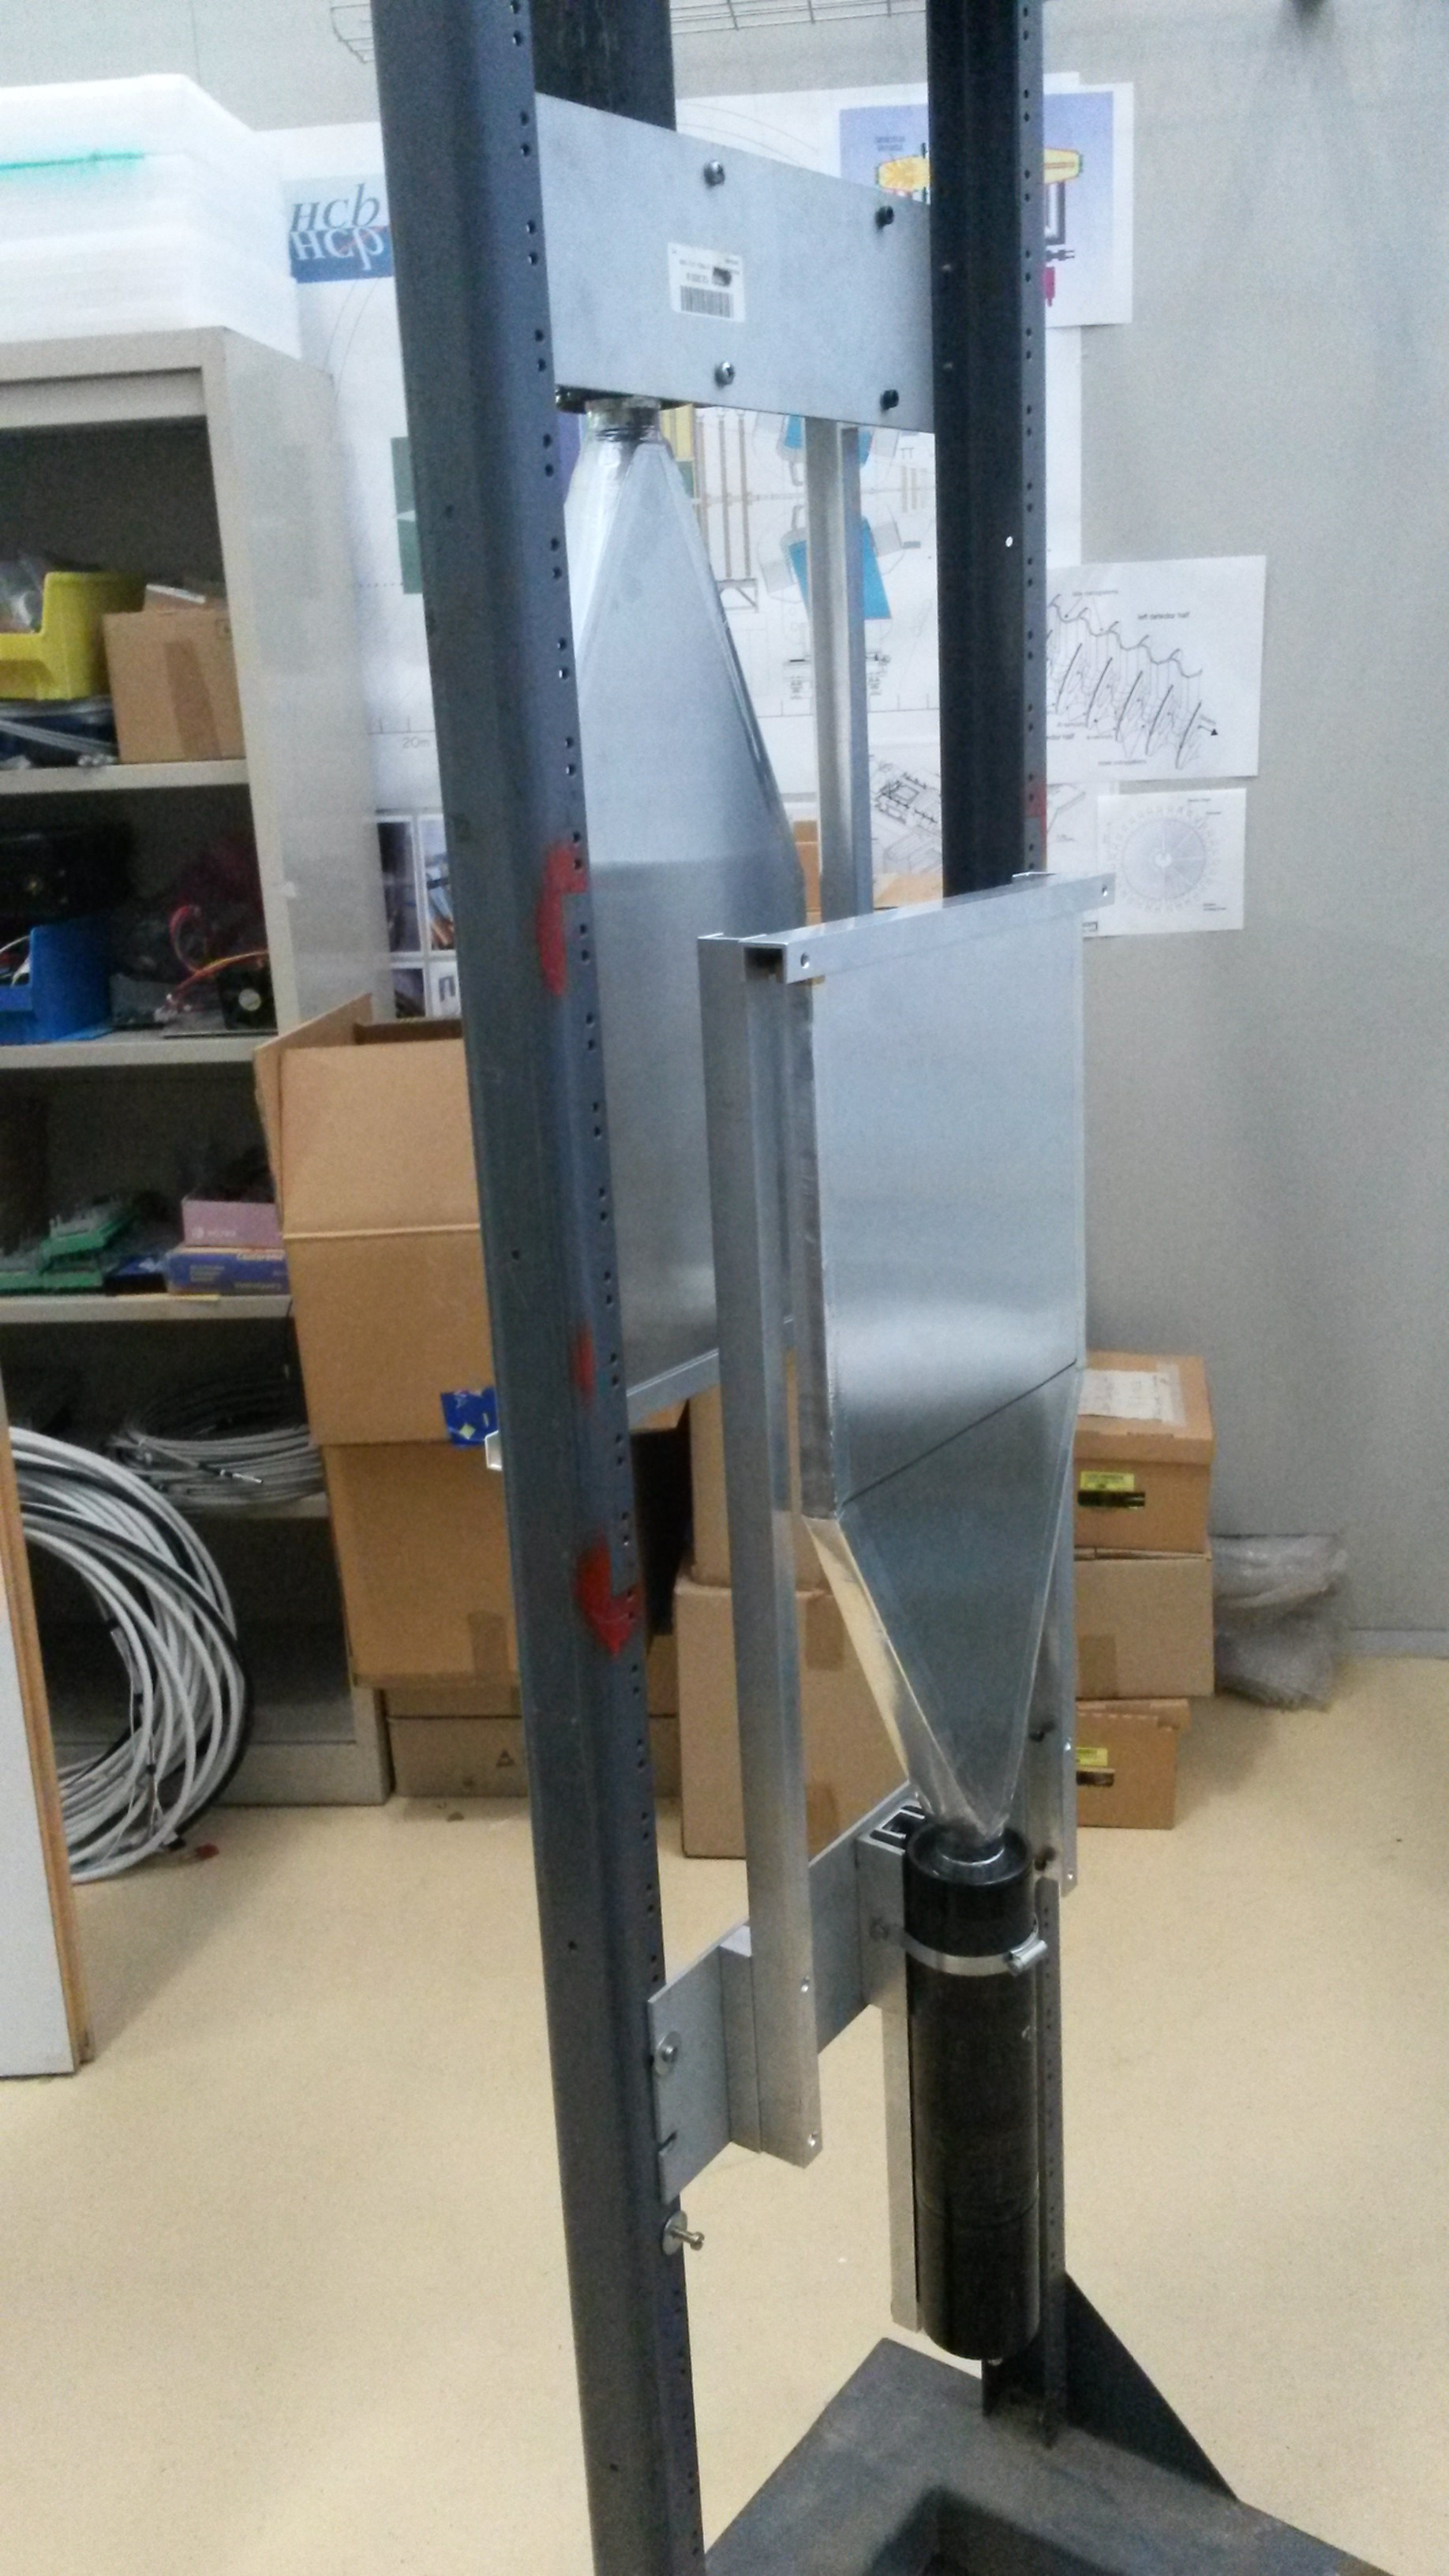
\includegraphics[width=0.8in]{figs/intro/mechanical_stand_1}
    \end{columns}
}


\frame{
    \frametitle{Background studies: measurements (cntd.)}
	\begin{itemize}
		\item Setup tested with cosmics. $\mathcal{O}(3000)$ triggers in a couple of hours.
	\end{itemize}
    \vspace{0.3cm}
	\begin{columns}
		\column{0.7\textwidth}
	    \centering
\includegraphics[width=2.3in]{figs/intro/codexb_test}		
         \column{0.3\textwidth}
          \centering
         {\scriptsize 1500~V bias}\\
         \includegraphics[width=1.4in]{figs/intro/HV1500}
    \end{columns}
    \vspace{0.3cm}
	\begin{itemize}
	\item Hope to get get enough events within around a week in the cavern. 
\end{itemize}
}



\section{Physics reach and planning}


\frame{
   \frametitle{Snapshot of benchmark scenarios}
   \begin{itemize}
   	\item Evolving situation depending on what timing, calorimetry, PID capabilities of the final detector will be.   	
   	\vspace{0.3cm}
   	\item Some benchmark scenarios: \vspace{0.3cm}
   \begin{itemize}
   	\item Light GeV-scale \textcolor{red}{scalar $\varphi$} (Higgs mixing)
   	\vspace{0.4cm}
   	\item Massive \textcolor{red}{dark photons $\gamma_{\rm d}$} from exotic Higgs decays (kinematic mixing)
   	\vspace{0.4cm}
   	\item \textcolor{red}{Heavy Neutral Leptons}, (mixing w/ SM neutrinos)
   	\vspace{0.4cm}
   	\item \textcolor{red}{Dark glueballs}, \textcolor{red}{axion like particles} (need calorimetry for $\gamma$ modes)
   	\end{itemize}
   \end{itemize}
   \begin{center}
   	{\small (present reach plots from D. Robinson {\em et al.})}
   \end{center}
}

\frame{
   \frametitle{$b\to s \varphi$ Higgs-scalar mixing}
	\centering
\includegraphics[width=4.5in]{figs/intro/codexb_phi_reach}		
   \begin{itemize}
   	\item Extends LHCb reach considerably and covers large part of MATHUSLA/SHiP reach.
   \end{itemize}
}

\frame{
	\frametitle{Dark photons from $h\to\gamma_{\rm d}\gamma_{\rm d}$ decays}
	\centering
	\includegraphics[width=3.1in]{figs/intro/codexb_h2gdgd}		
	\begin{itemize}
		\item Extends LHCb reach and at low masses (large boosts), coverage beyond ATLAS.
	\end{itemize}
}

\frame{
  \frametitle{HNL's: $U_{\ell N}$}
	\centering
\includegraphics[width=4.7in]{figs/intro/codexb_hnl}		
\begin{itemize}
	\item Different reaches/constraints for $\ell\in \{e, \mu, \tau\}$
	\item Dominated by charm/B decays at low/high masses.
\end{itemize}  
}

\frame{
	\frametitle{Mass resolution}
     \begin{itemize}
     	\item CODEX-b should also be able to do mass analysis depending on tracking + timing resolutions [1705.06327, Curtin/Peskin]
     	\item Require minimum 6 hits/daughter track. Shown for $B\to X\varphi$:
     \end{itemize}
     \begin{center}
     \includegraphics[width=3.7in]{figs/intro/mass_res}     	
     \end{center}


}
\frame{
	\frametitle{Todo's: near and long-term future}

	\begin{itemize}
		\item Studies for physics reach + BG measurements are on track.
		\vspace{0.3cm}
		\item Realistic \textcolor{red}{simulation + tracking} in {\tt DD4Hep}.
		\vspace{0.3cm} 
		%\item Options for (inexpensive) fast timing? Can we gain from HL collider technology sans radiation hardness?
		\vspace{0.3cm}
		\item \textcolor{red}{Detector technologies}: options for 4d timing+tracking in low radiation/background environment? \textcolor{red}{Calorimetry} options?
		%\vspace{0.3cm}
		%\item Main USP is, it's an inexpensive detector.
    \end{itemize}
\pause
	\begin{center}
	\includegraphics[width=4.7in]{figs/intro/codexb_timeline}
\end{center}
}

\frame{
	\frametitle{CODEX-b: Who we are}
	\begin{itemize}
		\item \textcolor{red}{Theory} colleagues:\\ \hspace{0.5cm} {\small S. Knapen, M. Papucci, D. Robinson}
		\vspace{0.4cm}
		\item \textcolor{red}{LHCb} physicists:\\ \hspace{0.5cm} {\small V. Coco, B. Dey, R. Dumps, V. Gligorov, H. Schindler, \\ \hspace{0.5cm} T. Szumlak, X.~Vidal~ + many others...}
		\vspace{0.4cm}
		\item Growing collaboration...you're very welcome to join!!! 
	\end{itemize}
\pause
\vspace{0.3cm}
\begin{center}
	{\Large {\em Thanks!}}
\end{center} 
}
